\documentclass{../main.tex}[subfiles]
\begin{document}
\chapter{Introduzione}
In questo capitolo presenterò gli aspetti matematici fondamentali per andare ad affrontare gli argomenti del corso.
\\
\section{Vettori e matrici}
Denotiamo un vettore riga e colonna rispettivamente con $(a,b,c)$ e $ \begin{bmatrix} a \\ b \\ c \end{bmatrix} $
\\dove $a,b,c\in\mathbb{R}$ sono scalari.
\\
In generale denotiamo con le lettere maiuscole le matrici, e.g. $X$ e i suoi elementi con $X_{ij}$.\\
$x\in \mathbb{R}^n$ è un vettore di n elementi e $X \in \mathbb{R}^{m \times n}$ è una matrice di dimensione $m \times n$.
\section{Norme di vettori e matrici}
Dato un vettore $x\in \mathbb{R}^n$ vi sono diversi tipi di norme comunemente utilizzate.
\begin{itemize}
	\item $||x||_2=(\sum_{i=1}^n x_i^2)^{\frac{1}{2}}$
	è il tipo più comune e viene chiamato \textbf{norma 2} di un vettore o \textbf{norma Euclidea}. Normalmente è denotato semplicemente con $||x||$.
	\item $||x||_1=|x_1|+|x_2|+\cdots+|x_n|$, detta la \textbf{norma 1} o \textbf{distanza di Manhattan}
	\item $||x||_\infty=\max_{1\leq i\leq n}|x_i|$, detta la \textbf{norma $\infty$}.
\end{itemize}
Analogamente, per una matrice $X \in \mathbb{R}^{m \times n}$, si possono definire diverse norme:

\begin{itemize}
	\item \textbf{Norma di Frobenius}: $||X||_F = \left( \sum_{i=1}^m \sum_{j=1}^n |X_{ij}|^2 \right)^{\frac{1}{2}}$
	\item \textbf{Norma spettrale (o norma 2)}: $||X||_2$
	\item \textbf{Norma 1}: $||X||_1=\sum_{i,j} |X_{ij}|$
\end{itemize}
\section{Notazioni generiche}
Siano:
\begin{itemize}
	\item $u$: variabile indipendente (input), non necessariamente un vettore o uno scalare
	\item $v$: variabile dipendente (output), come sopra 
\end{itemize}
allora abbiamo che:
\begin{itemize}
	\item $x=\Phi(u)$, dove $x\in \mathbb{R}^d$ è il vettore di features e $\Phi$ è la funzione di mapping o embedding.
	\item $y=\Psi(v)$, dove $y\in \mathbb{R}^m$ è il vettore target (o di output) e $\Psi$ è la funzione di mapping di feature in output.
\end{itemize}
Siano $x^1,\dots x^n$ e $y^1,\dots y^n$ due dataset di $n$ esempi, dove $x^i$ e $y^i$ formano la $i$-esima coppia di dati. Dunque $n$ è il numero di campioni, allora posso associarvi le due matrici dei dati
$$X=\begin{bmatrix}
	(x^1)^T\\ \vdots \\ (x^n)^T
\end{bmatrix}\in \mathbb{R}^{n \times d}, \quad Y=\begin{bmatrix}
	(y^1)^T\\ \vdots \\ (y^n)^T
\end{bmatrix}\in \mathbb{R}^{n \times m}$$
Le cui righe sono i vettori feature e i vettori target rispettivamente, trasposti.\\
Definiamo allora:
\begin{itemize}
	\item $g_\theta: \mathbb{R}^d \to \mathbb{R}^m$ è un predittore. 
	\item $\hat{y}=g_\theta(x)$ è la predizione di $y$, dato $x$.
	\item $\Theta\in\mathbb{R}^p$ è il vettore di parametri del predittore.
\end{itemize}
La scelta dei parametri $\Theta$ a seconda dei dati viene chiamato \textit{training} o \textit{fitting} del predittore. 
\\
Separando le definizioni in base al dominio di riferimento, abbiamo le seguenti suddivisioni:
\begin{itemize}
	\item Spazio di input:
	\begin{itemize}
		\item Istanza (sample, oggetto, record): un esempio descritto da un certo numero di attributi.
		\item Attributo (campo, caratteristica, variabile): misura di un aspetto di una istanza.
	
	\end{itemize}
	\item Spazio di output:
	\begin{itemize}
		\item Classe (label, target): categoria a cui appartiene una istanza.
	\end{itemize}
	\item Predittore o modello:
	\begin{itemize}
		\item Una funzione $g$ con parametri $\Theta$ che dato uno spazio di input $X$ produce uno spazio di output $Y$.produce una predizione nello spazio di output $Y$.
	\end{itemize}
\end{itemize}

\begin{figure}[H]
	\centering
	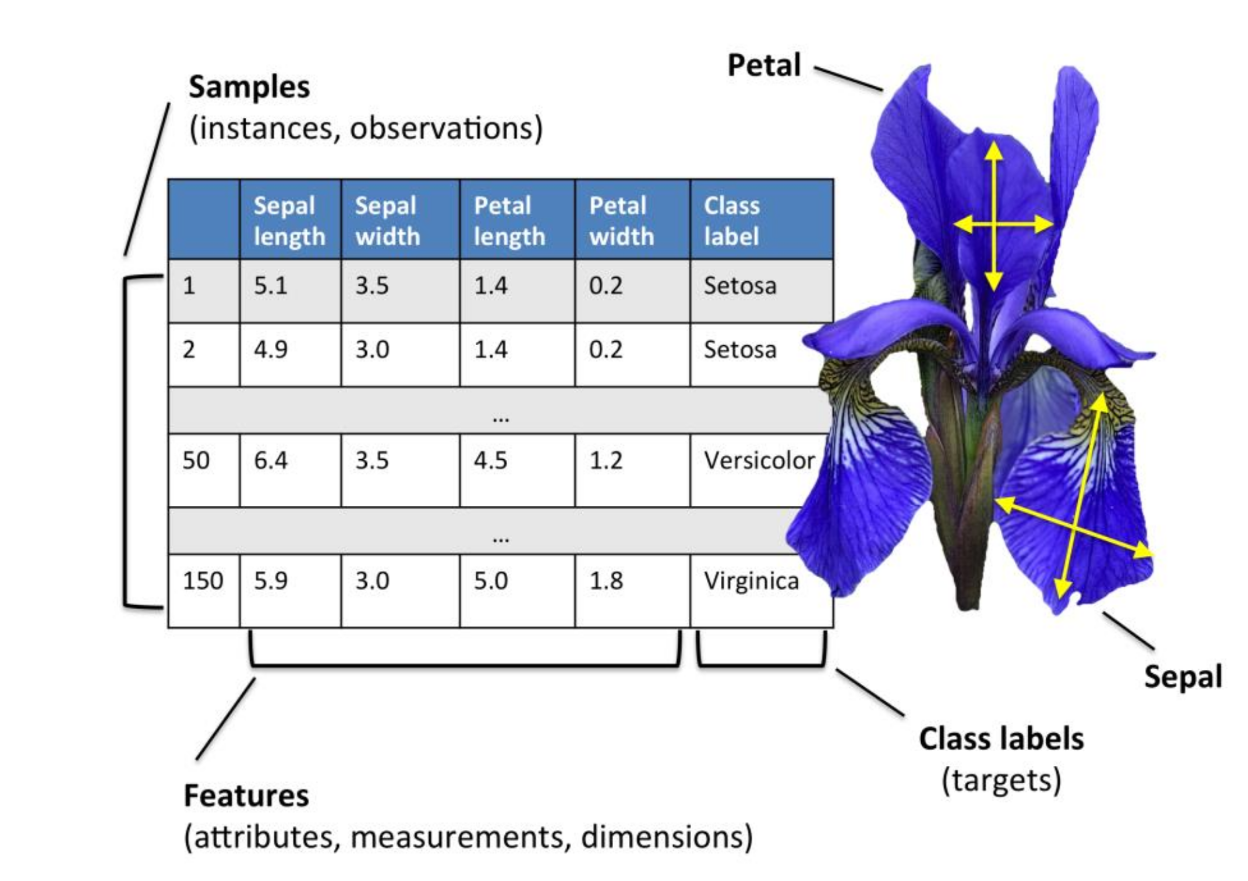
\includegraphics[width=0.6\textwidth]{pictures/esempioDefinizioni.png}
	\caption{Esempi pratici.}
\end{figure}
\begin{figure}[H]
	\centering
	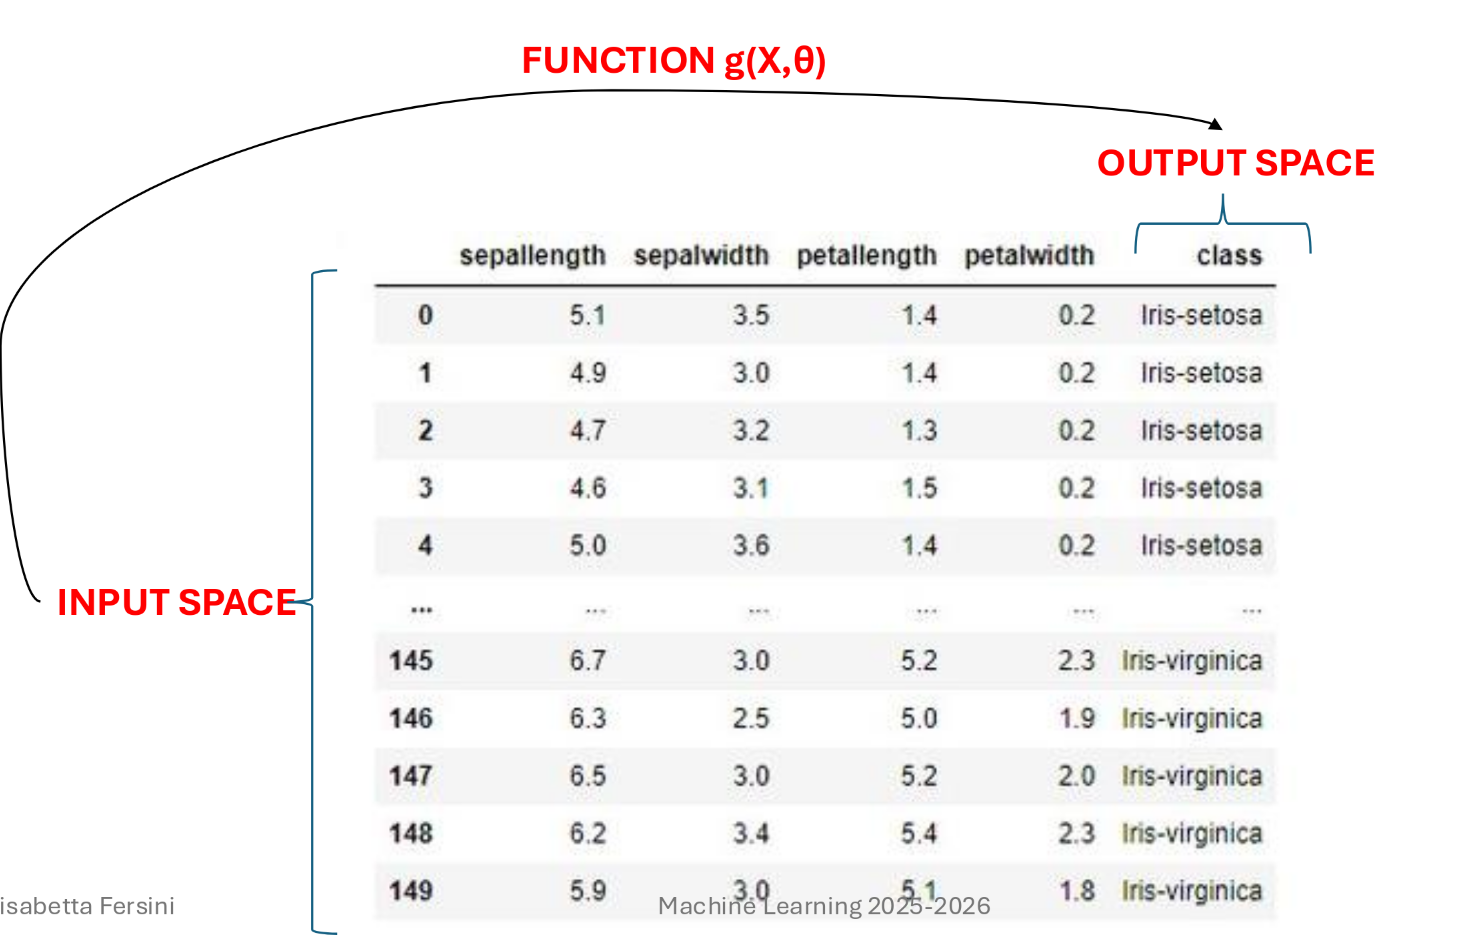
\includegraphics[width=0.6\textwidth]{pictures/esempioDefinizioni2.png}
	\caption{Esempi pratici 2.}
\end{figure}
\begin{figure}[H]
	\centering
	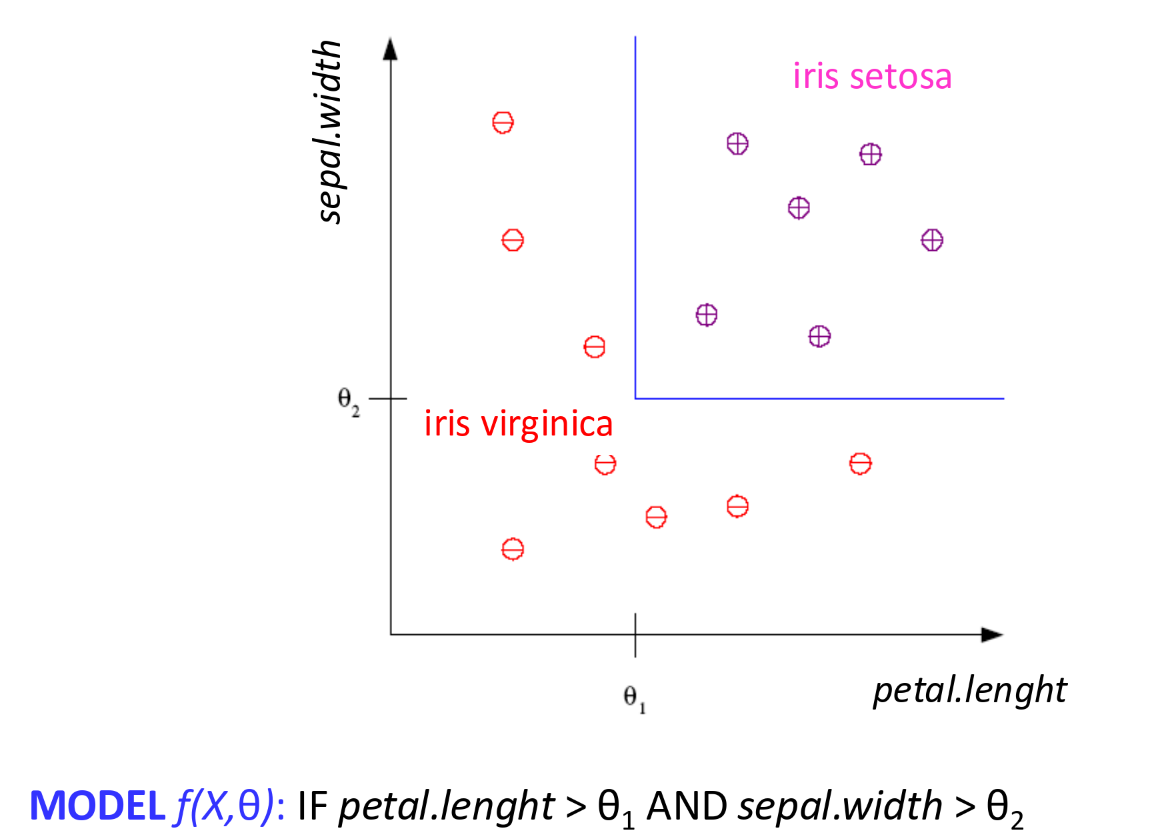
\includegraphics[width=0.6\textwidth]{pictures/esempioDefinizioni3.png}
	\caption{Esempi pratici 3.}
\end{figure}
\section{Rischio atteso e rischio empirico}
Quando un modello di machine learning $g$ viene addestrato, vogliamo che abbia buone prestazioni non solo per i dati utilizzati per il training, ma anche per dati sconosciuti (\textit{generalizzazione}).
Dovremo stimare il \textbf{rischio atteso}, ovvero la loss media che dovrebbe presentarsi sulla reale distribuzione dei dati $P(x,y)$. 
\\
Supponiamo di avere un dataset di $n$ coppie $(x^i,y^i)$, dove $x^i$ è il vettore di feature e $y^i$ il vettore target associato alla $i$-esima istanza.
Definiamo la \textbf{loss function} $L(g_\Theta(x),y)$, che misura l'errore commesso dal modello $g_\Theta$.
\\
Dunque il rischio atteso è definito come:
$$R(g_\Theta)=E_{(x,y)\sim P}[L(g_\Theta(x),y)]$$
Da notare però che la reale distribuzione $P$ \underbar{non è nota}, dunque non possiamo stimare il rischio atteso. Le cause sono:
\begin{enumerate}
	\item Distribuzione non nota \\
		Osserviamo solo un campione finito di campioni estratti dal mondo reale. La distribuzione completa che genera quei dati non è accessibile.
	\item Impossibilità pratica\\
		Anche se conoscessimo il processo di generazione in teoria, calcolare esattamente la predizione del rischio è impossibile in generale perché richiederebbe di sommare/integrare tutte i possibili esempi.
	\item Dati finiti e rumorosi\\
		Il dataset a disposizione è finito, spesso presenta rumore e errori di misura, o bias di raccolta. Dunque possiamo solo approssimare il rischio utilizzando una \textbf{stima empirica}.
\end{enumerate}
Dunque, vogliamo stimare e minimizzare il rischio empirico. Supponiamo di avere un dataset di $n$ coppie $(x^i,y^i)$.
Definiamo la loss function $L(g_\Theta(x),y)$, che misura l'errore commesso dal modello $g_\Theta$.
Allora il rischio empirico $\hat{R}(g_\Theta)$ è definito come:
$$\hat{R}(g_\Theta)=\frac{1}{n}\sum_{i=1}^n L(g_\Theta(x^i),y^i)$$
La maggior parte degli algoritmi di machine learning minimizzano il rischio empirico.
$$g^*=arg\min_{g_\Theta\in G}\hat{R}(g_\Theta)$$

\end{document}